\usetikzlibrary{arrows.meta,calc}
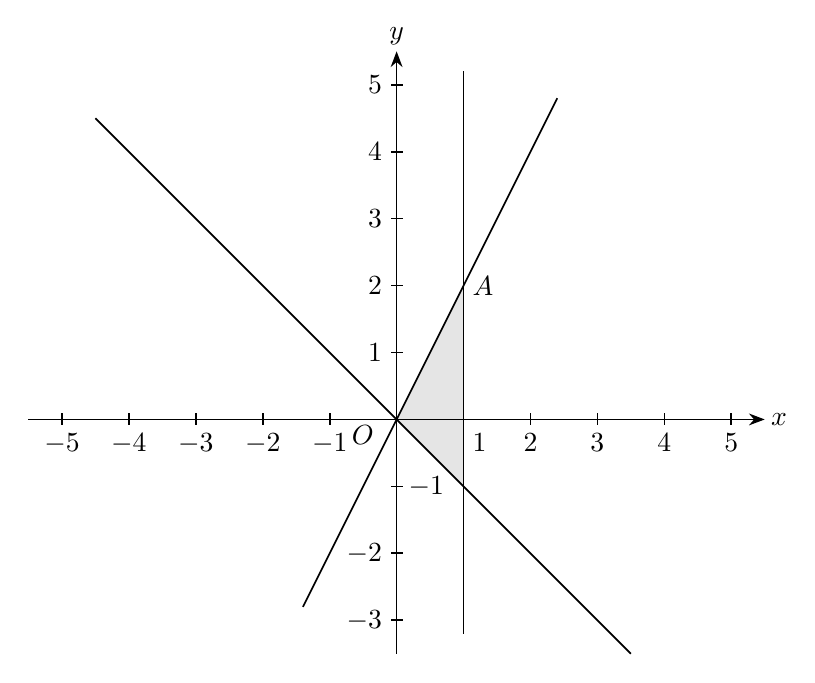
\begin{tikzpicture}[x=0.85cm,y=0.85cm,line width=.6pt,font=\normalsize,every node/.style={inner sep=0pt},>=Stealth]
% shaded triangle O(0,0)-A(1,2)-C(1,-1)
\fill[gray!20,draw=none] (0,0) -- (1,2) -- (1,-1) -- cycle;
% solid boundaries
\draw (-4.5,4.5) -- (3.5,-3.5);
\draw (-1.4,-2.8) -- (2.4,4.8);
\draw (1,-3.2) -- (1,5.2);
% axes
\draw[->] (-5.5,0) -- (5.5,0);
\draw[->] (0,-3.5) -- (0,5.5);
% integer ticks (no 0), numerals 2pt clear of axis
\foreach \t in {-5,-4,-3,-2,-1,1,2,3,4,5} {
  \draw (\t,0.09) -- (\t,-0.09);
  \ifnum\t=1
  \node[below right,inner sep=0pt,xshift=3pt,yshift=-5pt] at (\t,0) {$\t$};
  \else
  \node[below=5pt,inner sep=0pt] at (\t,0) {$\t$};
  \fi
}
\foreach \t in {-3,-2,-1,1,2,3,4,5} {
  \draw (0.09,\t) -- (-0.09,\t);
  \ifnum\t=-1
  \node[right=4pt,inner sep=0pt] at (0,\t) {$\t$};
  \else
  \node[left=5pt,inner sep=0pt] at (0,\t) {$\t$};
  \fi
}
% labels (O hugs origin, clear of -1 tick glyphs; A clears x=1 and slant line)
\node[below left,inner sep=0pt,xshift=-8pt,yshift=-2pt] at (0,0) {$O$};
\node[right=2pt,inner sep=0pt] at (5.5,0) {$x$};
\node[above=2pt,inner sep=0pt] at (0,5.5) {$y$};
\node[right=3pt,inner sep=0pt] at (1,2) {$A$};
\end{tikzpicture}
